\documentclass[letterpaper, 12pt]{article}
\usepackage{pgfplots}
\usepgfplotslibrary{fillbetween}
\pgfplotsset{compat=1.13}

\title{Basics of Economics}
\author{Alvin Lin}
\date{Principles of Microeconomics: August 2016 - December 2016}

\begin{document}

\maketitle

\section{Output and Costs}

\subsection{Factors of Production}
Factors of production are the raw materials and various other components
required to produce a good. These can include factories and machines, workers,
physical resources, time, and technology.

\subsection{The Time Horizon}
When we look at the time horizon, there are two distinct segments: the ``short
run'', and the ``long run''. The factor which seperates these two segments is
simple: in the short run, at least one factor of production is firm, meaning
its effect on production is unchangeable. In the long run, however, all factors
are variable, meaning there are no permanent restrictions on the flow of
production.

\subsubsection{Example}
Say we want to produce muffins. We would require the following:
\begin{itemize}
  \item A factory building, which takes six months to build or procure.
  \item At least one worker, which takes at least two weeks to find and hire.
  \item Ovens, which take three days to ship from the manufacturer to your
        location.
\end{itemize}
In this scenario, the short run horizon is six months, as after six months
all of this listed factors will be, or at least could be, developed, meaning
they are no longer fixed and we have entered the long run portion of the
time horizon.

\subsection{Fixed Costs}
A fixed cost is a cost that must be paid regardless of the quantity produced,
and does not increase or decrease according to this quantity. The lease on
the factory from the previous example is an example of a fixed cost. This is
the cost of any firm factor of production.

\subsubsection{Total Fixed Cost (TFC)}
Total Fixed Cost is the sum of all fixed costs in the production process.

\subsection{Variable Costs}
Variable costs are dynamic costs which vary according to the quantity of a
good produced. The flour required to produce a single muffin in the previous
example represents a factor which has a variable cost, as each additional
muffin produced requires another bit of flour to produce.

\subsubsection{Total Variable Costs (TVC)}
Total Variable Cost is the sum of all variable costs in the production process
at a certain level \( p \).

\subsection{Total Cost}
The total cost of the production process is:
\[ TC(p) = TFC+TVC(p) \]

\subsubsection{Example}
\begin{center}
  \begin{tabular}{|c|c|c|c|c|}
    \hline
    Laborers & Muffins & TFC & TVC  & TC  \\ \hline
    0        & 0       & 25  & 0    & 25  \\ \hline
    1        & 4       & 25  & 25   & 50  \\ \hline
    2        & 10      & 25  & 50   & 75  \\ \hline
    3        & 13      & 25  & 75   & 100 \\ \hline
    4        & 15      & 25  & 100  & 125 \\ \hline
    5        & 16      & 25  & 125  & 150 \\ \hline
  \end{tabular}
\end{center}
In this chart, marginal benefit applies with the principle of diminishing
returns. The threshold is at three workers, after which the marginal
contribution of additional workers begins to decrease.
\begin{center}
  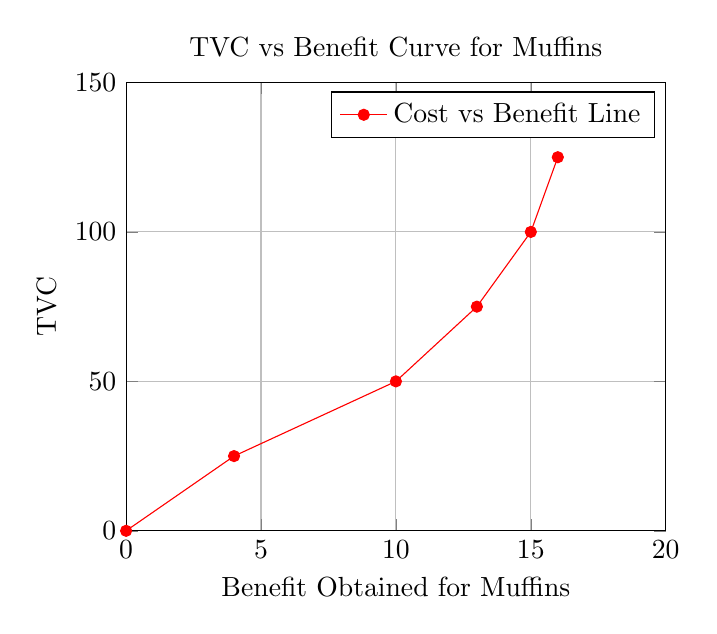
\begin{tikzpicture}
    \begin{axis} [
      title={TVC vs Benefit Curve for Muffins},
      xlabel={Benefit Obtained for Muffins},
      ylabel={TVC},
      xmin=0, xmax=20,
      ymin=0, ymax=150,
      grid=both
    ]
    \addplot[color=red, mark=*] coordinates {
      (0,0) (4,25) (10,50) (13,75) (15,100) (16,125)
    };
    \addlegendentry{Cost vs Benefit Line}
    \end{axis}
  \end{tikzpicture}
\end{center}

\subsection{Average Total Cost (ATC)}
The average total cost of the production process is:
\[ ATC(p) = \frac{TVC(p)}{p} \]
On the graph, the slope of the tangent line to the curve represents the
average total cost. As \( p \) becomes larger, \( ATC(ρ) \) converges on
\( TVC(p) \), until they eventually become arbitrarily close. At first,
\( ATC \) will be decreasing, because additional workers will still have an
increasing marginal contribution. However, there exists a point \( p^{*} \),
where \( AVC = TVC \). This point represents the point at which additional
workers yield a diminishing return.

\subsection{Marginal Cost Rules}
The marginal cost is the increase in total cost at the \( p \)th unit.
\begin{enumerate}
  \item If \( ATC > MC \), then \( ATC \) is decreasing.
  \item If \( AVC > MV \), then \( AVC \) is decreasing.
  \item If \( ATC < MC \), then \( ATC \) is increasing.
  \item If \( AVC < MC \), then \( AVC \) is increasing.
  \item If \( ATC \) is minimized, then \( ATC = MC \).
  \item If \( AVC \) is minimized, then \( AVC = MC \).
\end{enumerate}

\begin{center}
  If any errors are found, please contact me at alvin.lin.dev@gmail.com
\end{center}

\end{document}
